\section{Boltzmann correction and physical consistency}
\label{sec:boltzmann}

The Maxwellian baseline of Section~\ref{sec:baseline} returns
$\beta_{\mathrm{Max}} = 14.27\,$ms together with
$\varepsilon_{\mathrm{Max}} = 7.73\times10^{-30}\,$m\,atom$^{-1}$
and reproduces both anchor etch rates to machine precision. The
residual physical problem is that the fitted $\beta$ is between a
factor of 2.5 and 100 smaller than any gas residence time accessible
to the target reactor class at $10\,$mTorr. The identifiability
analysis of Section~\ref{sec:identifiability} leaves only one degree
of freedom in which the discrepancy can live---the
rate-source-dependent product entering the invariant
\eqref{eq:invariant-full}---and the obvious candidate within that
product is $\kdiss$ itself.

The kinetics data set used throughout this work contains, in
addition to the Maxwellian rate coefficients obtained by convolving
the Biagi cross sections \citep{biagi} with a Maxwell--Boltzmann
distribution at the tabulated $T_e^{\mathrm{eff}}(E/N,x_{\mathrm{Ar}})$,
a parallel set of rate coefficients obtained by solving the two-term
Boltzmann equation for the same cross sections on the same
$(E/N,x_{\mathrm{Ar}})$ grid using BOLSIG$^+$ \citep{hagelaar2005}.
Both rate families are aggregated over identical sets of process
labels, so the only difference between them is the EEDF used to
compute the rate integral. The reduced model accepts either rate
source through a dispatch branch in the kinetics backend with no
other changes to the pipeline: replacing the Maxwellian rate source
with the Boltzmann rate source is a controlled one-variable
experiment whose only effect is to substitute three scalars
($\kiz$, $\katt$, $\kdiss$) at the calibration operating point.

A potential concern with this procedure is that the two anchor
measurements are taken in different reactors and that any
chamber-to-chamber systematic would appear in the calibrated
parameters regardless of the rate source used. This concern does
not affect the comparison reported here: both the Maxwellian
calibration of Section~\ref{sec:baseline} and the Boltzmann
calibration of the present section use the identical pair of anchor
data points, so any systematic shift introduced by chamber-to-chamber
differences enters both calibrations identically and cancels
exactly from the ratio
$\beta_{\mathrm{Bolt}}/\beta_{\mathrm{Max}}$ that the identifiability
invariant predicts. The absolute values of $\beta$ and
$\varepsilon$ may inherit unknown chamber-specific offsets, but the
rate-source-dependent shift that is the subject of
Sections~\ref{sec:boltzmann}--\ref{sec:observability} is independent
of those offsets.

At $E/N = 100\,$Td and $x_{\mathrm{Ar}} = 0$, the two rate sources
give
$\kiz^{\mathrm{Max}} = 2.39\times10^{-19}$ vs
$\kiz^{\mathrm{Bolt}} = 9.31\times10^{-26}\,$m$^3$\,s$^{-1}$,
$\katt^{\mathrm{Max}} = 3.46\times10^{-15}$ vs
$\katt^{\mathrm{Bolt}} = 4.28\times10^{-15}$, and
$\kdiss^{\mathrm{Max}} = 1.109\times10^{-17}$ vs
$\kdiss^{\mathrm{Bolt}} = 3.804\times10^{-19}$. The Maxwellian
assumption overestimates $\kiz$ by seven orders of magnitude,
overestimates $\kdiss$ by a factor of 29.2, and leaves $\katt$
within $24\,\%$ of the Boltzmann value. The pattern follows from
the structure of the \sfsix{} EEDF in the attachment-dominated
regime: the two-term Boltzmann distribution has its high-energy
tail strongly suppressed relative to a Maxwellian at the same mean
energy, so electron-impact processes that integrate against the
tail are sharply reduced while attachment (dominated by electrons
below $1\,$eV) is approximately preserved. The full rate ratios
across the $E/N$ range are shown in Fig.~\ref{fig:rate-ratios}.

\begin{figure}[t]
  \centering
  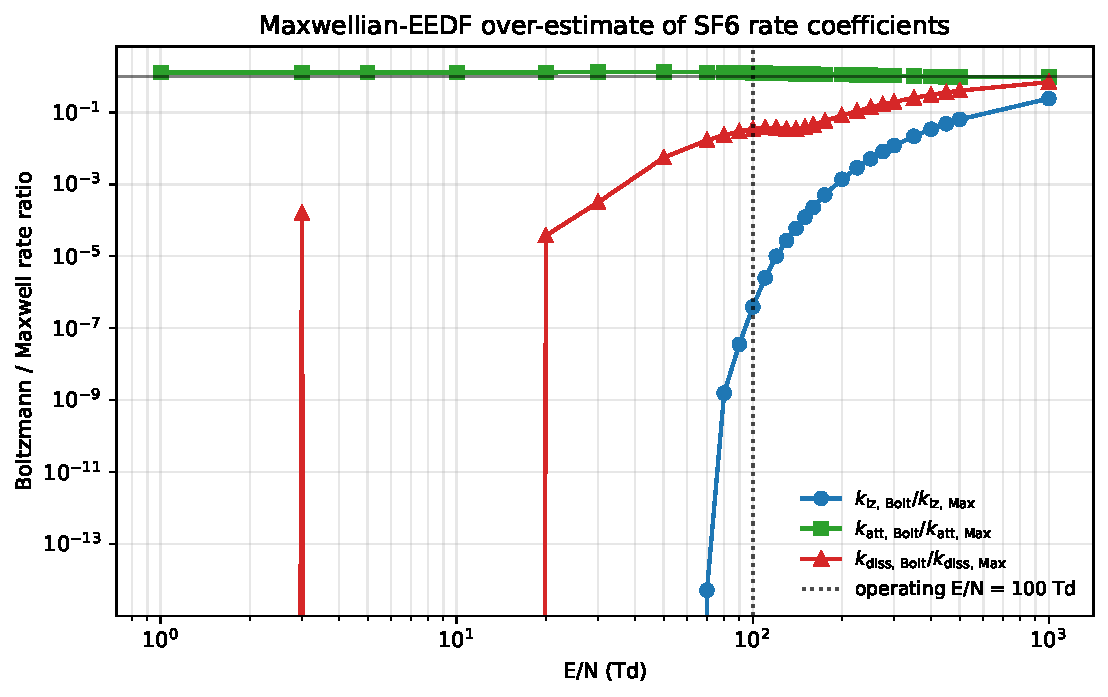
\includegraphics[width=0.8\linewidth]{figures/fig2_rate_ratios}
  \caption{Maxwellian-to-Boltzmann rate-coefficient ratios for
  \sfsix{} across the reduced-field range. At the operating point
  $E/N = 100\,$Td (vertical dotted line), the Maxwellian assumption
  overestimates $\kdiss$ by a factor of $29.2$ and $\kiz$ by seven
  orders of magnitude, while $\katt$ is within $24\,\%$ of the
  Boltzmann value. Aggregated from the Biagi SF$_6$ cross-section
  set \citep{biagi} using BOLSIG$^+$ \citep{hagelaar2005}.}
  \label{fig:rate-ratios}
\end{figure}

Repeating the depletion calibration with the Boltzmann rate source
and leaving every other parameter untouched returns
$\beta_{\mathrm{Bolt}} = 509.22\,$ms and
$\varepsilon_{\mathrm{Bolt}} = 2.76\times10^{-28}$\,m\,atom$^{-1}$.
Both anchors are reproduced to within the numerical tolerance of
the fit. The self-consistent electron density at the high-power
anchor shifts modestly:
$\nel^{\mathrm{Bolt}}(P_H) = 1.285\times10^{19}\,$m$^{-3}$ against
the Maxwellian value
$\nel^{\mathrm{Max}}(P_H) = 1.574\times10^{19}\,$m$^{-3}$, a ratio
of $1.224$. The main numerical results of the two calibrations are
collected in Table~\ref{tab:boltzmann}.

\begin{table}[t]
\centering
\caption{Fitted depletion parameters and internal variables under
Maxwellian and two-term Boltzmann rate sources, with the pipeline
and calibration targets held identical.}
\label{tab:boltzmann}
\begin{tabular}{lcc}
\toprule
Quantity & Maxwellian & Boltzmann \\
\midrule
$\kdiss$ at $100\,$Td ($10^{-18}\,$m$^3$\,s$^{-1}$)
  & $11.09$ & $0.380$ \\
$\nel(P_H)$ at $2\,$kW ($10^{19}\,$m$^{-3}$)
  & $1.574$ & $1.285$ \\
$\varepsilon$ ($10^{-30}\,$m\,atom$^{-1}$)
  & $7.73$  & $276.0$ \\
$\beta$ (ms)
  & $14.27$ & $509.22$ \\
$\mathcal{I} = \beta\kdiss\nel(P_H)$
  & $2.491$ & $2.487$ \\
$r(200\,$W$)$ (nm\,min$^{-1}$)
  & $1400.00$ & $1400.00$ \\
$r(2000\,$W$)$ (nm\,min$^{-1}$)
  & $2270.00$ & $2270.00$ \\
\bottomrule
\end{tabular}
\end{table}

The ratio
$\beta_{\mathrm{Bolt}}/\beta_{\mathrm{Max}} = 35.68$ is the main
numerical result of the section, and it is quantitatively predicted
by the identifiability theorem of
Section~\ref{sec:identifiability}. Substituting the measured rate
ratios and $\nel$ shift into equation~\eqref{eq:beta-shift} gives
$\beta_{\mathrm{Bolt}}^{\mathrm{pred}}
= 14.27 \times 29.22 \times 1.224 = 509.22\,$ms, in agreement
with the refit to better than $0.5\,\%$. The naive form of the
invariant---$\beta\kdiss$ without the $\nel$ correction---predicts
$415.9\,$ms and leaves a $22\,\%$ residual; the full invariant
$\beta\kdiss\nel(P_H)$ recovers the fit exactly. Table~\ref{tab:boltzmann}
shows that the invariant $\mathcal{I}$ is preserved between the two
rate sources to 0.16\,\%, confirming that the rate-source-dependent
$\nel$ shift from the power balance is a necessary component of the
invariant rather than an auxiliary correction
(Fig.~\ref{fig:pred-residual}).

\begin{figure}[t]
  \centering
  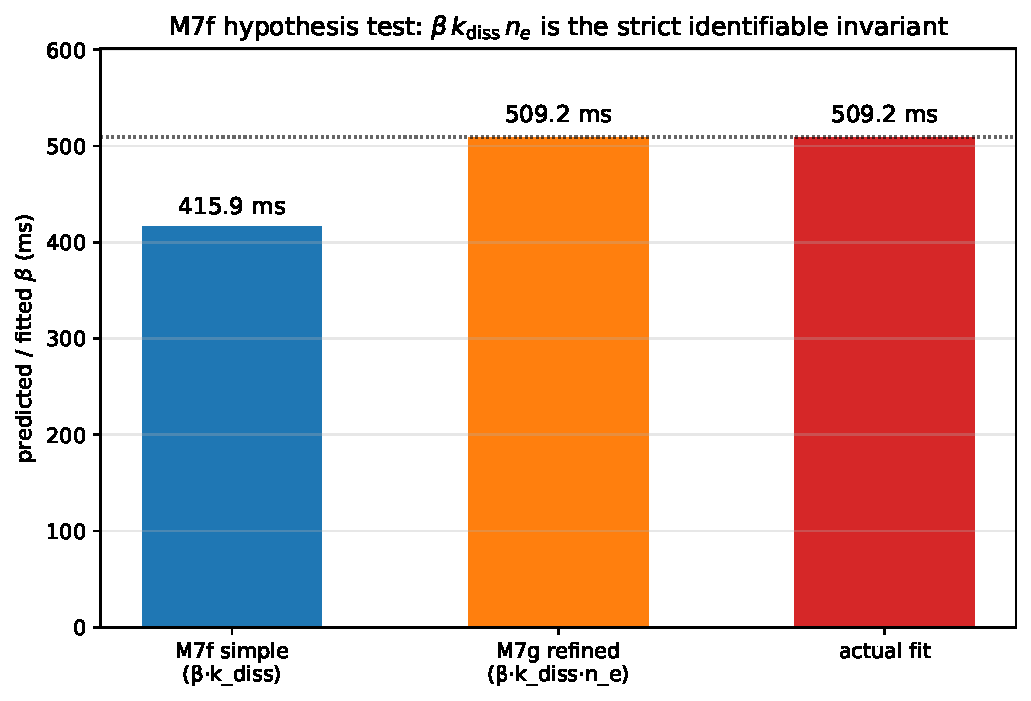
\includegraphics[width=0.78\linewidth]{figures/fig6_prediction_residual}
  \caption{Test of the identifiability invariant as a predictive
  tool. The naive prediction using $\beta\kdiss$ alone yields
  $\beta_{\mathrm{Bolt}}^{\mathrm{pred}} = 415.9\,$ms, off by
  $+22\,\%$. The refined prediction using the full invariant
  \eqref{eq:invariant-full}, including the secondary $\nel$ shift
  from the modified power balance, yields $509.22\,$ms, matching
  the direct Boltzmann refit to the tolerance of the numerical
  fit.}
  \label{fig:pred-residual}
\end{figure}

A second consistency check comes from comparing the Boltzmann-%
corrected $\beta_{\mathrm{Bolt}} = 509\,$ms against a nominal
geometric gas-phase residence time of a typical \sfsix{} ICP
reactor. For a cylindrical chamber of volume $V = 10\,$L at
$p = 10\,$mTorr and an inlet flow rate $Q_{\mathrm{in}}$ in the
commonly-used range $2$--$50\,$sccm, the geometric residence time
$\tau_{\mathrm{res}} \equiv \nSFsix\,V/\Gamma_{\mathrm{in}}$
spans $[36,\,1438]\,$ms. The Maxwellian value
$\beta_{\mathrm{Max}} = 14.3\,$ms lies more than a factor of 2
below this range and therefore cannot be interpreted as a residence
time under any reasonable flow rate; the Boltzmann-corrected value
$\beta_{\mathrm{Bolt}} = 509\,$ms falls within the range and is
consistent with residence times at moderate flow rates
(Fig.~\ref{fig:beta-validation}).

\begin{figure}[t]
  \centering
  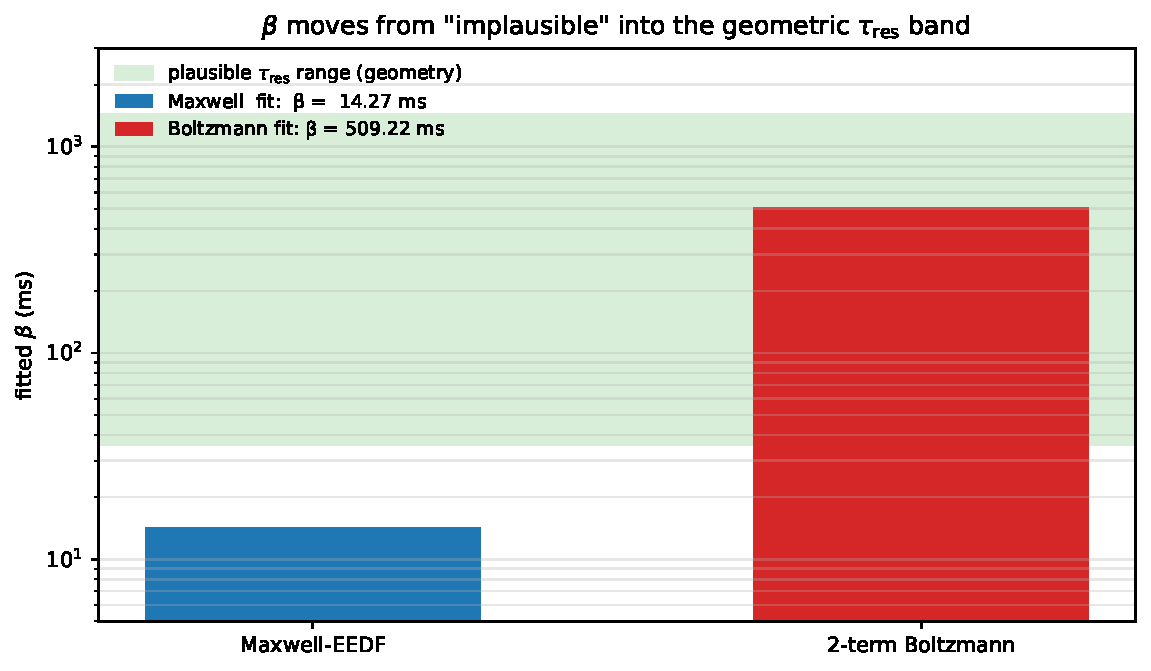
\includegraphics[width=0.78\linewidth]{figures/fig5_beta_validation}
  \caption{Fitted depletion timescale $\beta$ before and after the
  Maxwellian-to-Boltzmann rate-source correction, against the
  nominal geometric residence-time band
  $\tau_{\mathrm{res}}\in[36,1438]\,$ms (shaded). The Maxwellian
  value (blue) sits more than $2\times$ below the band and cannot
  be interpreted as a residence time; the Boltzmann value (red)
  lies within the band and is order-of-magnitude consistent.}
  \label{fig:beta-validation}
\end{figure}

We stress that this is a consistency check, not a direct
identification of $\beta$ with a physical residence time. The two
anchor measurements come from chambers of different geometry
operated at different pressures ($10\,$mTorr and $30\,$mTorr; see
Section~\ref{sec:baseline}), and the residence-time band quoted
here is a nominal range at the $10\,$mTorr calibration condition. A
single fitted $\beta$ with the model's lumped, zero-dimensional
feedstock balance cannot resolve chamber-to-chamber differences in
volume, pumping speed, or recirculation. What the comparison does
establish is that the Maxwellian fit produces a number that is
physically impossible as a residence time, while the Boltzmann fit
produces a number that is at least order-of-magnitude consistent
with residence-time physics. Under either interpretation the
direction and magnitude of the correction ($\sim\!36\times$) is
the same and is the quantitatively predicted consequence of the
identifiability theorem, not an artifact of the residence-time
comparison.

The Maxwellian convolution remains a standard shortcut in reduced
ICP models because for noble gases and near-equilibrium discharges
the rate-coefficient integral is insensitive to the shape of the
high-energy tail. For attachment-dominated electronegative plasmas
the tail is strongly depleted relative to a Maxwellian at the same
mean energy, and the error on individual rate coefficients
propagates multiplicatively through the identifiability manifold
into the fitted parameters. A fitted depletion or transport
parameter whose physical interpretation one wishes to trust must
therefore be preceded both by an identifiability analysis and by a
rate-source validation step. In the absence of either, the fitted
values may retain predictive power at the calibration operating
point without carrying any defensible physical interpretation.

Finally, the Boltzmann correction leaves the calibrated model's
predictions at the anchor operating condition unchanged by
construction: both modes hit both anchors exactly, and the
identifiability theorem guarantees that they agree to within the
tolerance of the numerical fit at every intermediate power along
the calibration $E/N$ as well (Fig.~\ref{fig:etch-comparison}).
What the correction changes is the point on the
$(\beta,\kdiss,\nel)$ manifold that the calibration lands on. The
observational question of whether the Maxwellian or Boltzmann rate
source corresponds to the physically realized state is therefore
not resolved at the calibration anchors; it is an off-anchor
observability question, which we take up in
Section~\ref{sec:observability}.

\begin{figure}[t]
  \centering
  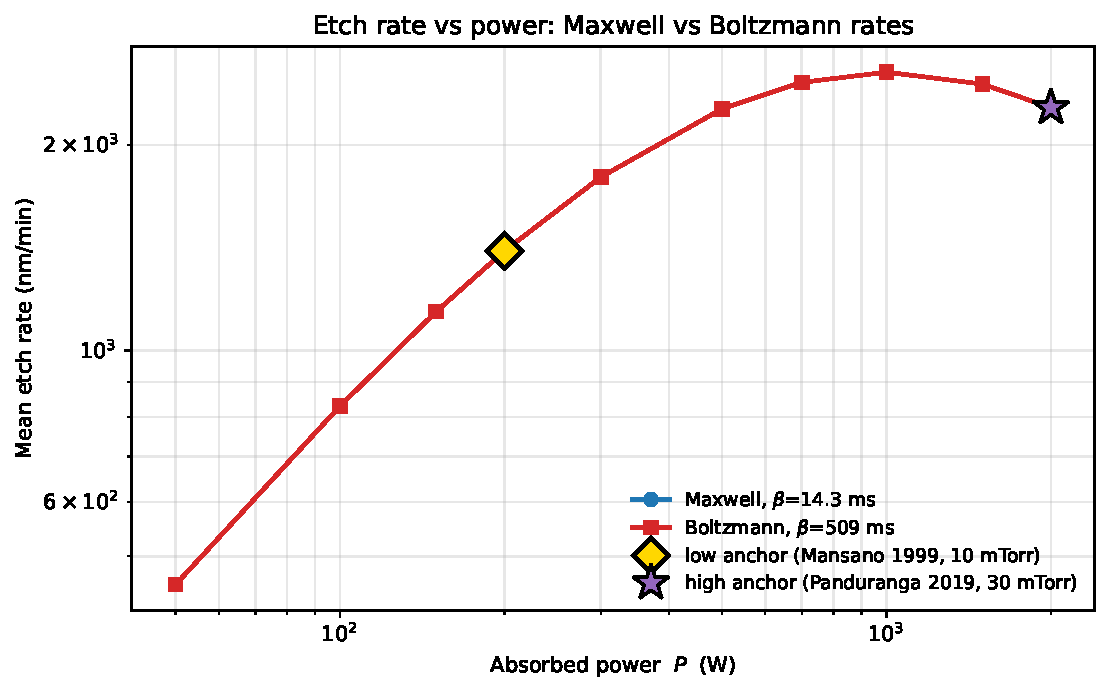
\includegraphics[width=0.78\linewidth]{figures/fig3_etch_comparison}
  \caption{Etch rate vs absorbed power at the calibration condition
  ($E/N = 100\,$Td, $x_{\mathrm{Ar}} = 0$, $p = 10\,$mTorr) for the
  Maxwellian-calibrated (blue) and Boltzmann-calibrated (red)
  models. Both curves pass through the Mansano~1999 ($10\,$mTorr,
  $200\,$W) and Panduranga~2019 ($30\,$mTorr, $2000\,$W) anchors
  by construction and are indistinguishable to the tolerance of
  the numerical fit at every intermediate power, a structural
  consequence of the identifiability theorem of
  Section~\ref{sec:identifiability}.}
  \label{fig:etch-comparison}
\end{figure}
